\section{Method}
\label{sec:method}

This thesis aims to produce a working implementation of an application with visual as well as natural-language input, using \gls{ttr}.
Such an application largely resembles those put forward in \cite{ttrspat} and \cite{lspc}, but there are some differences.
This application will feature:

\begin{enumerate}
\item Sensory input in the form of 2D images
\item Utilizing an external object recognition system
\item Detection of geometric spatial relations
\item Basic natural language understanding
\end{enumerate}

While operational functionality and the overall procedural code is written in Python, the core model is written in \gls{ttr} (realized as Python code using PyTTR).
As such, \gls{ttr} serves as a formal specification language.
The additional layer provides formal transparency and type robustness.

This section will describe some reasoning around the decisions taken, regarding the design of the \gls{ttr} model as well as its implementation.



\subsection{Object detection with YOLO}

You only look once (YOLO) \citep{RedmonYouOnlyLook2015} is a neural network model for image recognition.
It is trained using a loss function which takes detection as well as classification into account.
In other words, it simultaneously predicts bounding boxes and classifies the contained objects.
Unlike \cite{HeMaskRCNN2017} and others, it does not contain any recurrent layers.
The joint, recurrence-free model makes for a rather small network size, which in turn means a favorable evaluation speed.
However, compared to state of the art, it lags behind in accuracy.
The network is pretrained on the COCO dataset \cite{LinMicrosoftCOCOCommon2014}.

\begin{figure}[h]
\label{fig:dogbike_annotated}
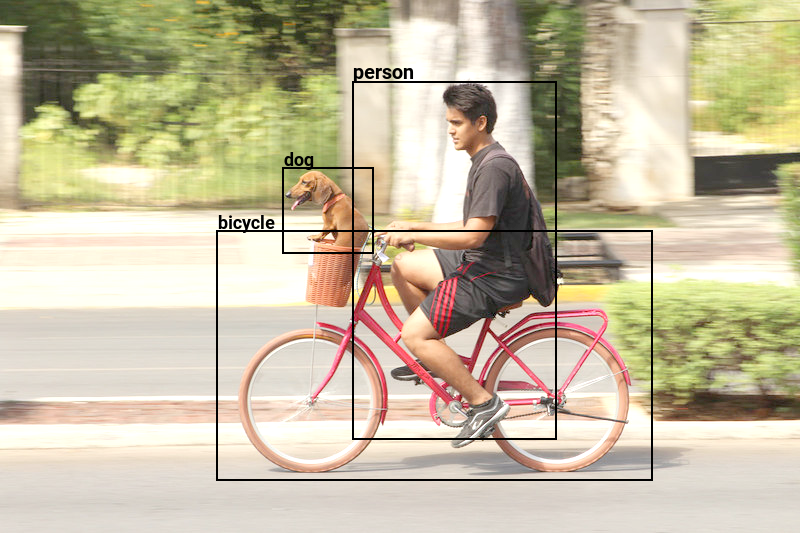
\includegraphics[width=\textwidth]{dogbike_annotated}
\centering
\caption{Visualization of the labels and bounding boxes emitted by YOLO when given an image depicting a cyclist with a dog.}
\end{figure}

YOLO is written in C, using the Darknet neural network library \citep{darknet13}.
It can be used in Python with the TensorFlow machine learning library and the Darkflow library which translates a Darknet model to TensorFlow.

When invoked from Python, the return value is a collection of dict objects, each containing a label, coordinates and a confidence score, as exemplified in \autoref{lst:yolo_out}.
Results with confidence over a certain threshold are cast into \gls{ttr} records as described in \autoref{ssec:python}.
In this process, the bounding box coordinates are cast from a top-left and bottom-right tuple $\langle\langle x_1, y_1\rangle, \langle x_2, y_2\rangle\rangle$ to a center-width-height tuple $\langle x_c, y_c, w, h\rangle$, as the latter is more adequate for spatial classification.

\begin{lstlisting}[label=lst:yolo_out, caption=Example output of YOLO invocation]
[
	{
		'topleft': {'x': 354, 'y': 86},
		'bottomright': {'x': 551, 'y': 437},
		'label': 'person',
		'confidence': 0.80116189
	},
	{
		'topleft': {'x': 224, 'y': 234},
		'bottomright': {'x': 646, 'y': 476},
		'label': 'bicycle',
		'confidence': 0.85828924
	},
	...
]
\end{lstlisting}



\subsection{Objects and perception}

Our model of the perception of objects is largely based on \cite{lspc}.
First, the object detection algorithm returns a set of \textit{perceptual objects}.
Each of them is evidence that a certain location is associated with a certain property (such as being a dog), but it does not constrain any individual to this association.
Second, an \textit{individuated object} is generated for each perceptual object.
This describes the situation that there is an individual, which has the given property, at the given location.
In the \gls{ttr} implementation (presented in full in \autoref{ssec:ttrmodel}), the individuated object is a type.
%[what's so good about it being a type?] \cite{BarwiseSituationsAttitudes1981}

In \cite{lspc}, the world has the form of a 3D point space rather than a 2D image.
This necessitates different types for the perceptual input and the locations of perceived objects.
In the point space case, the $PointMap$ set type is used for the full ``world'', and any part of the world is simply a subset of it, so it is also a $PointMap$.
In our case, $Image$ is used for the full image but we use $Segment$ to refer to parts of it.



\subsection{Spatial relations}
\label{sec:method-spatrel}
% Classification algorithm non-TTR. Simplistic, compare to sophisitcated alternatives.

Our method of spatial relation classification is inspired by \cite{ttrspat} but more simplistic.
One simplification is that the reference frame is fixed.
This means we only consider the deictic meaning of spatial relation terms, and not the intrinsic.
``Left'' will mean to the left in the plane of the image, even if the reference object is turned on the side or toward the viewer.

Another simplification is the neglection of the \textit{functional} aspect of spatial relations.
To illustrate this aspect, an umbrella may be well said to be \textit{above} a man, but less clearly \textit{over} him, if it does not protect him from rain falling sideways in hard wind \citep{CoventryInterplayGeometryFunction2001}.

In our model, a spatial classifier $\kappa$ takes two locations and returns a boolean result.
We have implemented spatial classifiers as Python functions.
For the purpose of this thesis, no sophisticated spatial classification has been considered.
Instead, a naive comparison between centers of bounding boxes was implemented.
This was done for the four relations ``left'', ``right'', ``above'' and ``below''.



\subsection{Language and \gls{vqa}}
\label{ssec:languagevqa}

In contrast to full \gls{vqa} systems, the model presented in this thesis will be restricted to a limited type of questions, namely polar questions on the location of one object in relation to another.
For example: ``Is the bicycle below the tree?''
A \textit{scene type} describing the visual scene is created by combining the types generated by the perceptual classification outlined above.
It serves as the context in which questions are evaluated.

The existing research on \gls{ttr}-based approaches to textual or phonetic parsing, overviewed in \autoref{ssec:ttnlp}, would surely cover the kind of utterances considered here.
However, there is currently no implementation available and ready to use, and parsing is not within the main focus of this thesis.
Therefore, the natural-language parsing implemented for this thesis is instead a simplistic one.
It uses feature structure context-free grammar (FCFG) tools available in NLTK \cite{BirdNaturalLanguageProcessing2009} to parse text into \gls{fol} expressions.
With a custom function {\tt fopc\_to\_pyttr}, the \gls{fol} expressions are transformed to a TTR record type.
As an example, the question ``Is there a dog to the left of a car?'' is parsed into the type in \autoref{eq:uttex}.

\begin{equation}\label{eq:uttex}
\left[\begin{array}{rcl}
\text{x} &:& Ind\\
\text{y} &:& Ind\\
\text{c}_\text{dog} &:& \text{dog}(x)\\
\text{c}_\text{car} &:& \text{car}(y)\\
\text{c}_\text{left} &:& \text{left}(x, y)\\
\end{array}\right]\end{equation}

The fact that the natural-language utterance is given a representation in the same formal framework as the image allows comparing them to each other.
The situation described by the question type will be true if there is a witness of that type \cite{BarwiseSituationsAttitudes1981,CooperAustiniantruthattitudes2005}.
The scene type, on the other hand, is considered true by virtue of being generated by perceptual classification.
It follows that the question type is true if it is a supertype of the scene type.

So rather than looking for a witness to the question type, we formulate the problem as subtype/supertype checking.
However, the subtype relation requires matching field labels, which will not be the case here, as labels are generated on the fly.
Thus, the condition is reformulated to allow relabeling \citep[pp. 133–135]{CooperTypetheorylanguage2016}:

If $Q$ is the type of a polar question utterance and $S$ is the type of the scene, the answer is YES if there is a relabeling $\eta$ such that $S \sqsubseteq Q_\eta$, and otherwise it is NO.

%[classification before/after question]



%\subsection{Evaluation}

%The system is tested on a few sentences for a few images.
%...
